\chapter{Results}
\label{chap:results}
\section{Production prevision for a single turbine}
\label{sec:res_single}

The evaluation of the model for the simulation of a single plant with precise input data (see sec. \ref{sub:metho_single}) was carried out on the HydroRaon power plant operated by the company Ercisol \cite{ercisol}. It was rebuilt on the site of an old run-of-the-river plant, dismantled fifteen years ago. This production site was chosen in this study because of the availability of runoff data, plant parameters, and production data. However, its operation started recently (04-12-2017) and the first months of operation were a running in phase during which the plant underwent adjustments and did not operate to its full potential. \newline
Figure \ref{raon_map} shows the locations of the plant and the closest gauge station, with their parameters. Table \ref{prod_raon} gives the measured monthly production of the plant, as published by the company on their website, as well as the production simulated with the model, using the hourly runoff time series from the ``Banque Hydro'' \cite{eaufrance}. The production of April was calculated starting on the 12\textsuperscript{th}, when the plant started operating. The hourly production is represented in figure \ref{prod_raon_curve}.

\begin{table}[H]
\footnotesize
 \centering
 \caption{Monthly production of the HydroRaon plant \cite{ercisol}}
 \label{prod_raon}
 \begin{tabular}{l|c|c|}
  &Ercisol data&Model output\\
  Month&Measured [MWh]&Simulated [MWh]\\
  \hline
  April&37&61\\
  May&86&119\\
  June&66&\\
  July&29&\\
  August&17&\\
 \end{tabular}
\end{table}

\begin{figure}[H]
\centering
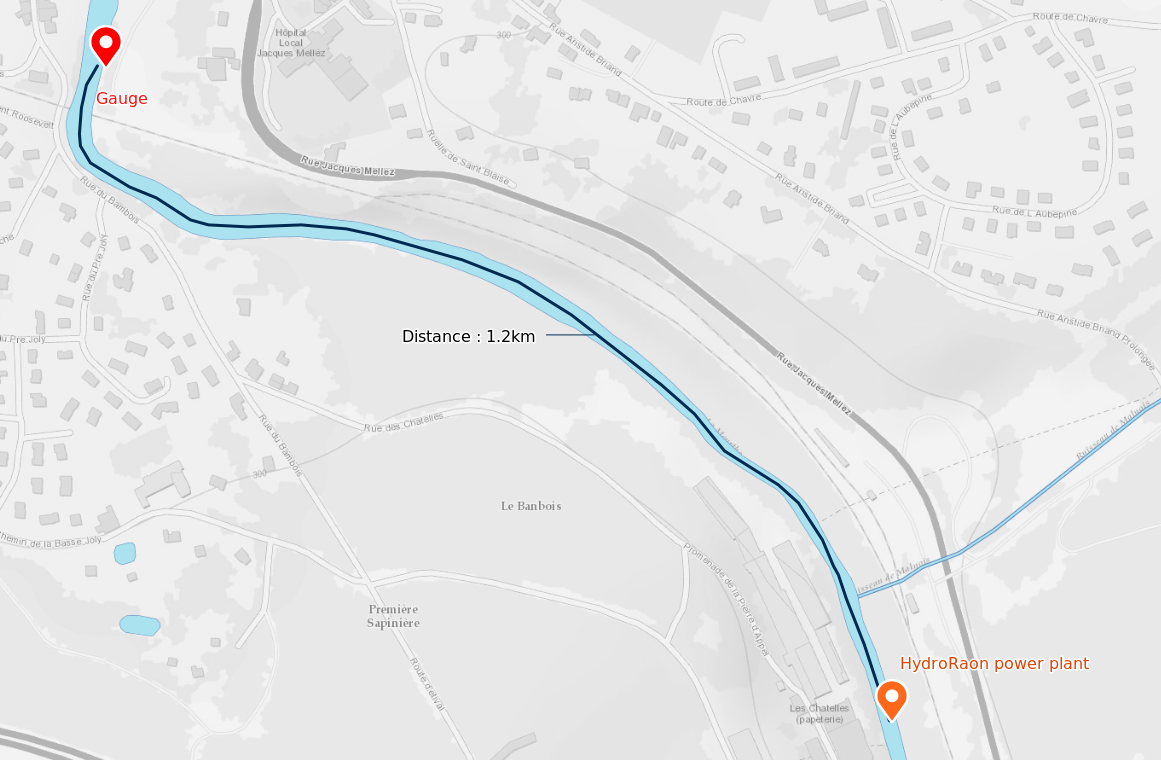
\includegraphics[width=14cm]{raon_map.png}
\caption{Sites and parameters of the HydroRaon plant and the Raon gauge station}
\label{raon_map}
\end{figure}

\begin{figure}[H]
\centering
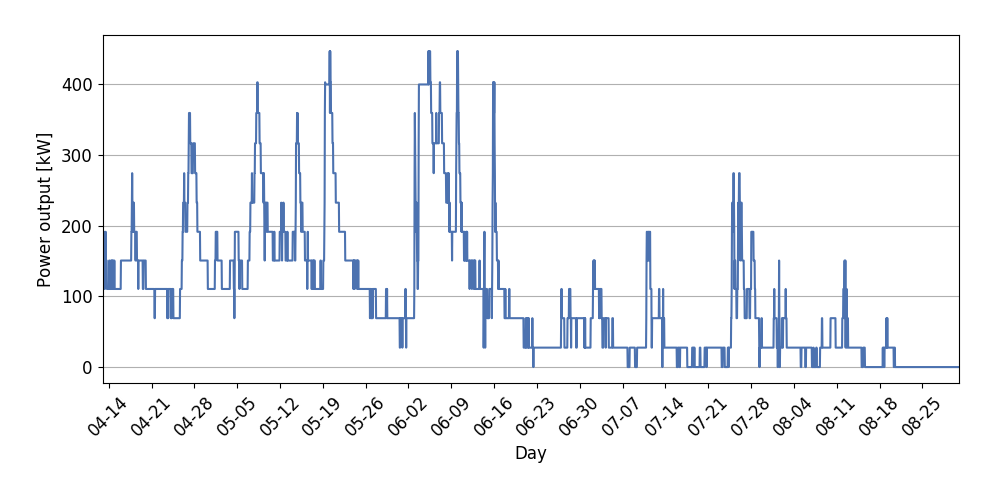
\includegraphics[width=10cm]{prod_raon_curve.png}
\caption{Simulated production of the HydroRaon plant}
\label{prod_raon_curve}
\end{figure}

The simulated production is significantly over the measured production of the plant. This could be due to the fact that the plant had just started operating and was undergoing a tests and adjustments. Unfortunately, at the time this work is being written, the measured runoff data from June to August is not yet available.

\section{Extrapolation of power plant data}
\label{missing_data}
Mosel : check that from Pnenn and flow values over several years we get Hn, Qn and turbine type

\section{Production prevision for a region}
\label{sec:res_th}

Sections \ref{sec:db_hydroelec} and \ref{sub:metho_sw} showed the problems inherent to comparing the results of a state-wide simulation based on the OpenEnergy Database with publicly available production data (from the Agentur für Erneuerbare Energien - AEE). Firstly, the AEE aggregates data from run-of-the-river plants, reservoir plants, as well as some pumped storage plants instead of differentiating them like the OpenEnergy Database. Secondly, the OEDB registers, in terms of number of plants and installed capacity, are not consistent with the AEE aggregated data, and the inconsistencies cannot be explained by the precedent remark alone. \newline
Section \ref{sub:metho_sw} justified the choice of running the state-wide simulation on the federal state of Thuringia and the results are presented here. \newline
The OEDB lists 205 run-of-the-river plants for Thuringia, displayed on figure \ref{map_th} along with the 18 used gauge stations, the average values of modeled runoff, and the river network.

\begin{figure}[H]
\centering
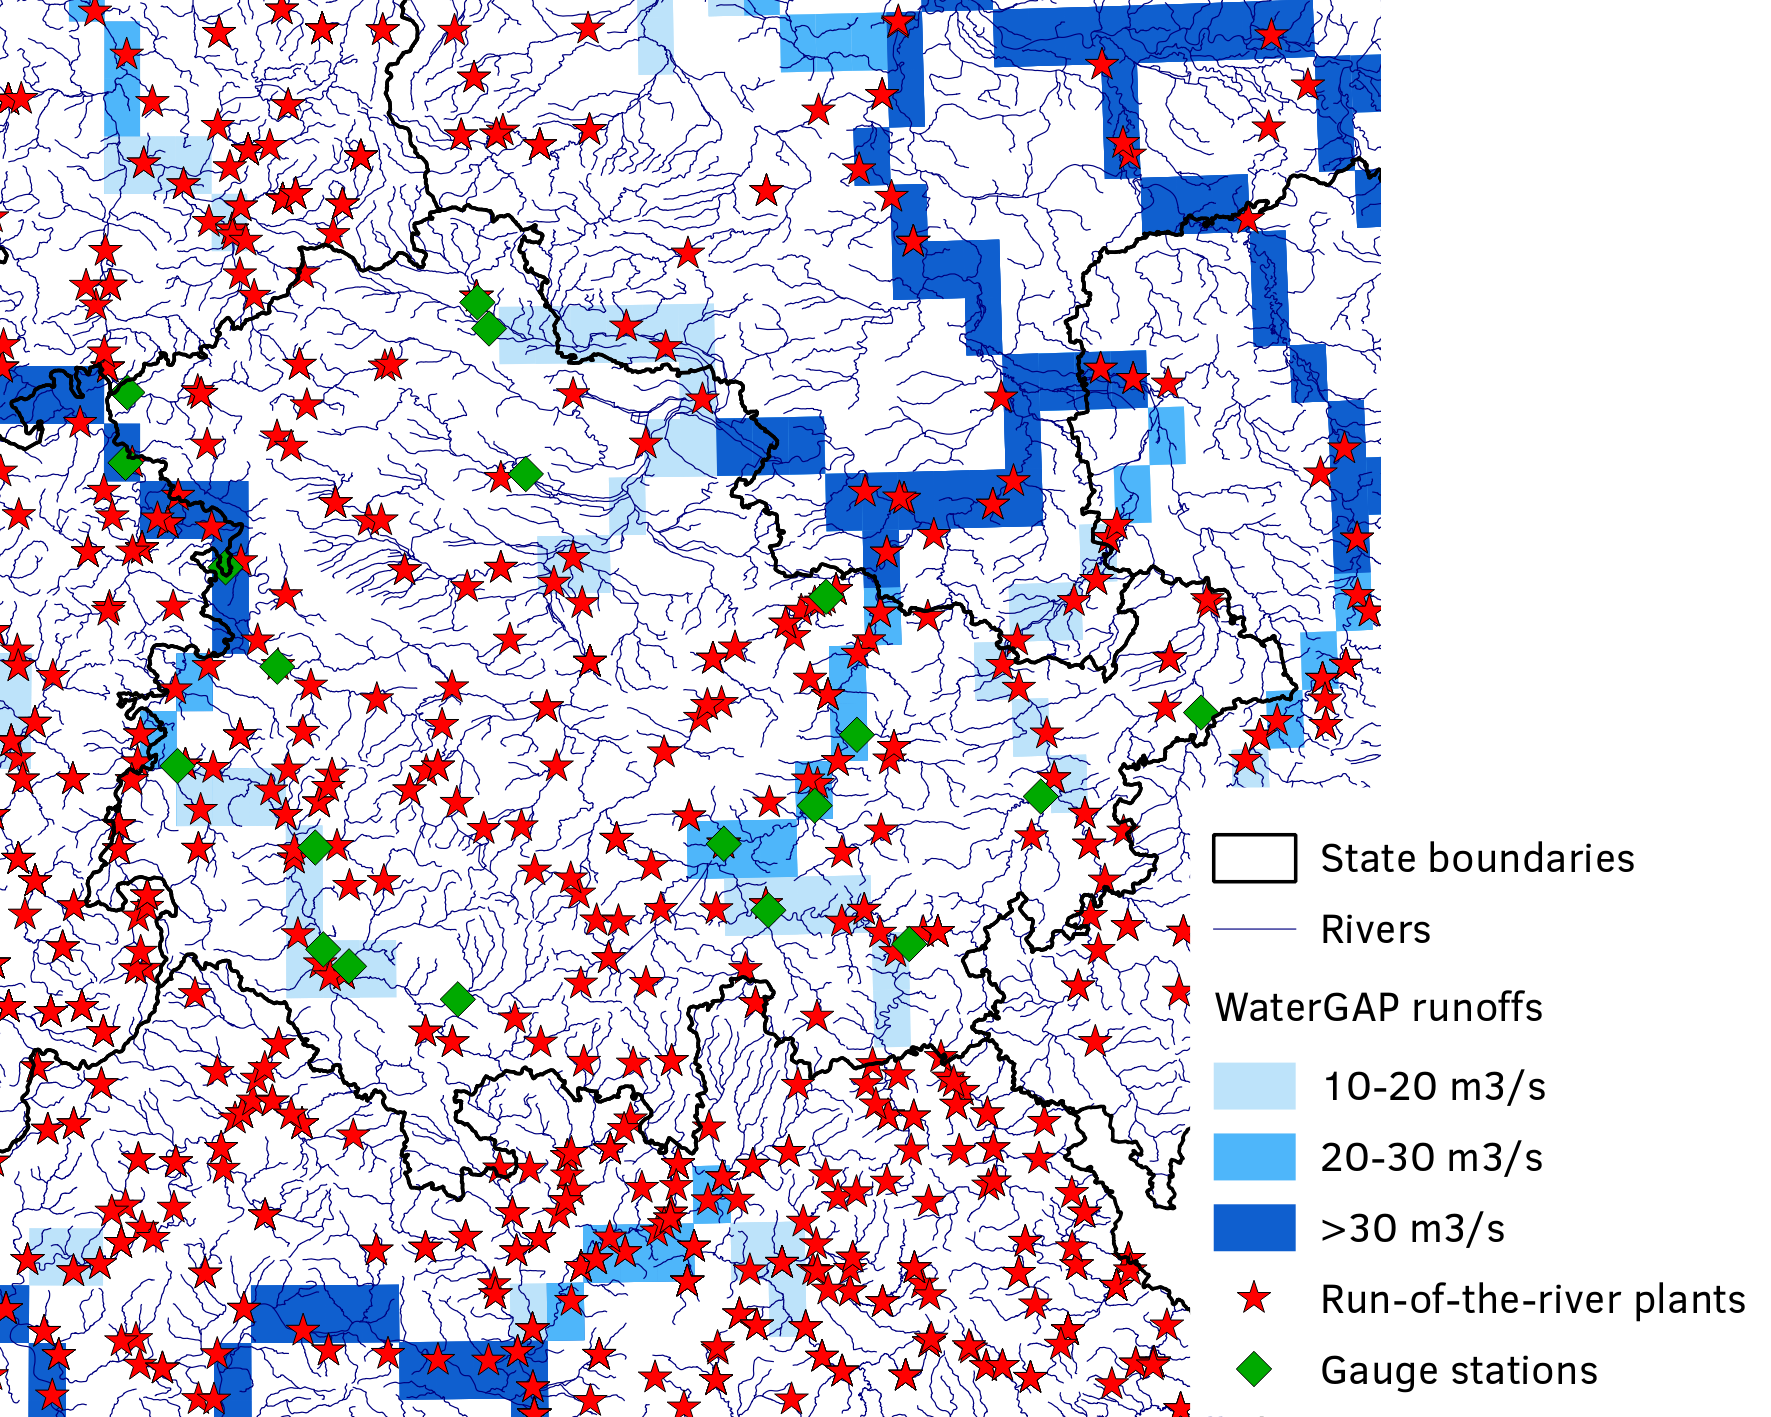
\includegraphics[width=15cm]{map_th.png}
\caption{Run-of-the-river plants, gauge stations, river and modeled runoff in Thuringia}
\label{map_th}
\end{figure}

To state-wide simulation were made : one based on modeled runoff and one based on measured runoff. The gauge assignment process described in section \ref{sub:pp_reg} could only assign gauge stations to 201 out of the 205 plants, therefore the simulations based on measured runoff were only run on these 201 plants.
